\documentclass[9pt,conference]{IEEEtran}
\usepackage[utf8]{inputenc}
\usepackage[brazil]{babel}

% Diversos
\usepackage{csquotes}
\usepackage{graphicx}
\usepackage{verbatim}
\usepackage{hyperref}
\usepackage{smartdiagram}

% Título
\title{Utilizando Redes Convolucionais de Grafos Espaço-Temporais para o Reconhecimento da Línguas de Sinais}
%\author{Cleison Correia de Amorim}
\date{Outubro 2018}

\author{
    \IEEEauthorblockN{Cleison Correia de Amorim}
    \IEEEauthorblockA{Centro de Informática\\
    Universidade Federal de Pernambuco\\
    Email: cca5@cin.ufpe.br}
}

% Comandos
% 'image': definição de imagem
\newcommand{\image}[4][\linewidth] {
    \begin{figure}[ht]
    \centering
    \includegraphics[width=#1]{#3}
    \caption{#4}
    \label{#2}
    \end{figure}
}

% 'refimage': referências de imagens
\newcommand{\refimage}[1] {figura \ref{#1}}

% 'refsection': referências de seções
\newcommand{\refsect}[1] {seção "\nameref{#1}"}

\begin{document}
\maketitle
\begin{abstract}
Este trabalho propõe a aplicação de um modelo de aprendizagem profunda baseado em grafos que descrevem o esqueleto humano afim de realizar a transcrição das características fonológicas da língua de sinais para uma representação em CORE-SL. Esse modelo de aprendizagem, conhecido como Rede Convolucional de Grafos Espaço-Temporais, é capaz de aprender automaticamente a partir dos padrões de movimentos humanos no espaço e no tempo representados por meio dos grafos.
\end{abstract}

%\begin{IEEEkeywords}
%Broad band networks, quality of service, WDM.
%\end{IEEEkeywords}


\section{Introdução} %%%%%%%%%%%%%%%%%%%%%%%%%%%%%%%%%%%%%%%%%%%
\label{sec:introducao}
Existe um grande número de estudos que propõem realizar a tradução da língua de sinais para sua equivalência na língua falada correspondente daquela região. Entretanto, muito desses estudos são limitados frente ao contexto cotidiano do Surdo por desconsiderarem aspectos relevantes da fonologia dessa língua como movimentos, expressões não-manuais, locação e orientação das mãos do interlocutor \cite{quadros-2004}. É comum também que tais estudos restrinjam seu campo de atuação ao âmbito da datilologia\footnote{
    Datilologia – também conhecida como alfabeto digital ou alfabeto manual. Consiste na soletração de palavras pelos Surdos. É geralmente utilizada para introduzir uma palavra que ainda não possui um sinal equivalente \cite{quadros-2004}\cite{pereira-choi-2011}.
}, que na prática é aplicada apenas em contexto restritos da comunicação desses indivíduos.

Em \cite{antunes-hcisl-2011}, os autores apresentam alguns outros fatores que ressaltam a limitação em trazer estudos assim para a realidade do Surdo: 
\begin{enumerate}
    \item O uso de equipamentos como luvas, acelerômetros e outros sensores que são de difícil acesso; 
    \item A adoção de métodos e tecnologias que não empatizam com a realidade Surdo, restringindo sua movimentação ou deixando de considerar aspectos importantes, como as expressões faciais;
    \item O uso de métodos que mapeiam sinais diretamente para palavras, e que tornam-se facilmente obsoletos mediante a introdução de novos sinais ou quando confrontados com variações linguísticas como gírias e regionalismos; 
    \item A utilização de imagens estáticas para o treinamento de modelos, que desconsideram a dinâmica da língua.
\end{enumerate}

Diante dessas limitações, foi introduzido em \cite{antunes-hcisl-2011} a proposta de uma arquitetura capaz de considerar os aspectos fonológicos da língua e de viabilizar a interação entre homem e máquina através de sinais, a qual foi denominada HCI-SL. A \refimage{fig:hcisl} apresenta essa arquitetura, onde uma API interna compreendendo tecnologias de visão computacional e processamento de linguagem natural proveem uma interface padrão para ferramentas e serviços externos como dicionários, tradutores e aplicativo de finalidades diversas.

\image
	[5cm]
    {fig:hcisl}
    {images/hcisl}
    {Arquitetura HCI-SL apresentada por \cite{antunes-hcisl-2011}.}

Contudo, para que a arquitetura acima funcionasse, foi necessário primeiro definir o CORE-SL, que consiste num modelo computacional para descrição dos sinais e suas características fonológicas. Ele estabelece um padrão de representação a ser adotado pelas peças que compõem a arquitetura HCI-SL.

De acordo com os autores, o CORE-SL:

\begin{quote}
[...] agrega flexibilidade e um nível de detalhamento capazes de proporcionar alternativas para um tratamento computacional robusto e para auxiliar às diferentes necessidades de aplicação. Este modelo atuará como um dos pilares de sustentação na construção de artefatos tecnológicos que considerem as necessidades deste perfil de usuário e tornem a comunicação usuário-sistema natural para ele. \cite{antunes-2011}
\end{quote}

 A \refimage{fig:coresl-interfaces} ilustra as interações do CORE-SL com um conjunto de serviços idealizados ou já em desenvolvimento por pesquisadores da Universidade Federal do Paraná - UFPR. Nela, o modelo exerce um papel central para a comunicação das peças envolvidas.

\image
    {fig:coresl-interfaces}
    {images/coresl_interfaces}
    {CORE-SL como peça chave para a comunicação entre serviços \cite{garcia-2013}.}

A \refimage{fig:coresl-sinalarvore}, por sua vez, mostra um exemplo de descrição do sinal "árvore" utilizando o CORE-SL.

\image
    {fig:coresl-sinalarvore}
    {images/sinal_arvore}
    {Representação do sinal árvore escrito segundo o CORE-SL.}
    

\section{Redes Convolucionais de Grafos Espaço-Temporais} %%%%%%%%%%%%%%%%%%%%%%%%%%%%%%%%%%%%%%%%%%%

Afim de viabilizar a transcrição dos sinais articulados pelo Surdo para o CORE-SL, fazia-se necessário selecionar uma técnica capaz de considerar os detalhes de diferentes partes do corpo humano e as nuances de seu movimento. Dessa forma, entre os diversos modelos analisados, optou-se pela escolha do \textit{Spatial-Temporal Graph Convolutional Networks - ST-GCN}\footnote{
    O código fonte do modelo ST-GCN é disponibilizado publicamente pelos autores no endereço \url{https://github.com/yysijie/st-gcn}.
} (ou Redes Neurais de Grafos Espaço-Temporais) proposto em \cite{st-gcn-2018}. Além dos fatores apontados anteriormente, tal escolha deve-se ao fato dele ser centrado na dinâmica do esqueleto humano e ser capaz de lidar com seu movimento sob duas perspectivas distintas e complementares entre si. Esses aspectos tornam a abordagem do ST-GCN extremamente relevante ao contexto da língua de sinais.

Segundo os autores:
\begin{quote}
A dinâmica dos esqueletos humanos transmite informações significativas para o reconhecimento de sua ação. Abordagens convencionais para modelagem de esqueletos geralmente dependem de partes feitas à mão ou de regras transversais, resultando assim em um poder expressivo limitado e dificuldades de generalização. [...] o ST-GCN vai além dessas limitações, aprendendo os padrões espaciais e temporais automaticamente a partir dos dados. Essa formulação não apenas conduz a um maior poder expressivo, mas também a uma capacidade de generalização mais forte \cite{st-gcn-2018}.
\end{quote}

O ST-GCN tem como base de sua formulação a sequência de grafos de esqueletos que representam o corpo humano, os quais são obtidos a partir de uma sequência de frames de vídeos de ações ordinárias desses indivíduos. A \refimage{fig:st-gcn-graph} permite-nos visualizar essa estrutura, onde cada nó corresponde a um ponto de articulação humano. Os vértices intra-corporais são definidos com base nas conexões naturais do corpo. Os vértices inter-frames, por sua vez, conectam as mesmas conexões (ou articulações) entre frames consecutivos para denotar sua trajetória no decorrer do tempo \cite{st-gcn-2018}.

\image
	[4cm]
    {fig:st-gcn-graph}
    {images/st_gcn_graph}
    {Sequência de grafos de esqueletos, que denotam o movimento humano no espaço e no tempo, utilizados pelo ST-GCN \cite{st-gcn-2018}.}

Para extrair a sequência de grafos descrita acima faz-se necessário aplicar uma etapa prévia de pré-processamento do \textit{dataset} denominada pelos autores como "estimação de pose". Nela, os autores fazem uso da biblioteca OpenPose\footnote{
	OpenPose - é uma biblioteca capaz de detectar os atores e fornecer cerca de 135 pontos referentes a partes de seus corpos, como mãos, braços e rosto. Disponível no endereço \url{https://github.com/CMU-Perceptual-Computing-Lab/openpose}.
} \cite{cao-realtime-2017}, \cite{simon-hand-2017}, \cite{wei-cpm-2016} e são capazes de extrair 18 pontos de articulação do corpo conforme apresentado na \refimage{fig:keypoints-pose}.

\image
	[4cm]
    {fig:keypoints-pose}
    {images/keypoints_pose_COCO_18}
    {Representação dos 18 pontos do corpo extraídos pelo OpenPose.}

A \refimage{fig:st-gcn-architecture} apresenta a arquitetura do modelo ST-GCN, que é essencialmente composta por 9 unidades de convolução espaço-temporal posicionadas de forma sequencial, e seguidas por uma camada de \textit{pooling} e um classificador \textit{softmax}.

\begin{figure}[ht]
    \centering
    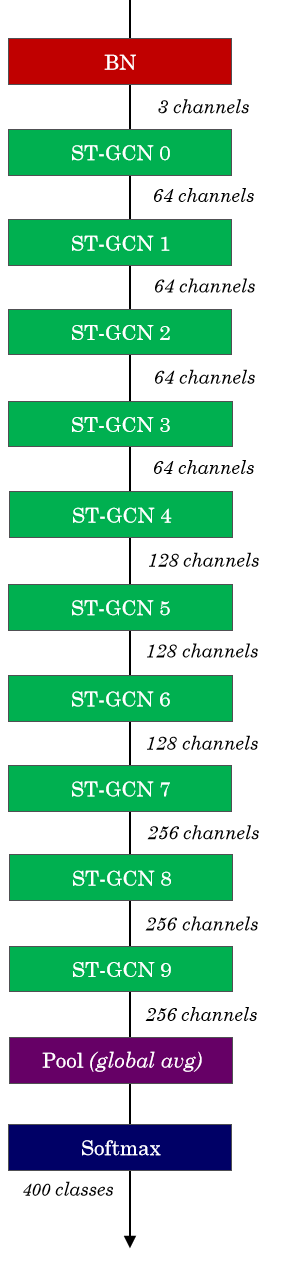
\includegraphics[width=3.2cm]{images/st_gcn_architecture}
    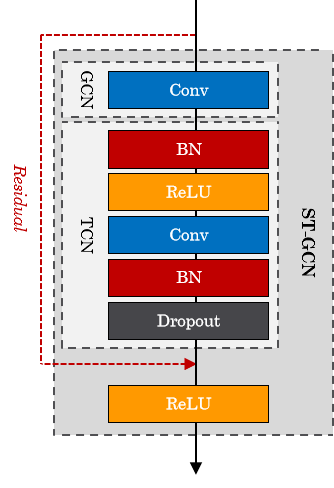
\includegraphics[width=3.5cm]{images/st_gcn_architeture_unit}
    \caption{Visão geral da arquitetura do modelo (à esquerda) e detalhe de uma unidade do ST-GCN (à direita).}
    \label{fig:st-gcn-architecture}
\end{figure}


\section{Dataset} %%%%%%%%%%%%%%%%%%%%%%%%%%%%%%%%%%%%%%%%%%%
\label{sec:dataset}
Será utilizado neste trabalho o \textit{dataset} \textit{American Sign Language Lexicon Video Dataset} (ASLLVD)\footnote{
    \textit{American Sign Language Lexicon Video Dataset} (ASLLVD) - disponível no endereço \url{http://vlm1.uta.edu/~athitsos/asl_lexicon/}
}, que dispõe de vídeos de sinais realizados por atores de diferentes níveis de proficiência na língua de sinais. Além disso, ele também disponibiliza os respectivos arquivos de metadados que determinam o nome e os respectivos frames de início e fim para os sinais contidos nos vídeos. É possível obter maiores detalhes acerca do \textit{dataset} em \cite{athitsos-asldataset-2008}.

\image
    {fig:asllvd-example}
    {images/asllvd_example}
    {Exemplo de representação do sinal \textit{"MERRY-GO-ROUND"} capturado em três perspectivas distintas no \textit{dataset} ASLLVD \cite{athitsos-asldataset-2008}.}

Para que os vídeos contidos no ASLLVD possam ser utilizados como entrada para o modelo ST-GCN, é necessário primeiro realizar um pré-processamento, que consiste nas seguintes etapas:
\begin{enumerate}
    \item Segmentar vídeos: as amostras do  ASLLVD compreendem seções onde foram gravados múltiplos sinais em sequência. Devido a isso, é necessário segmentá-los em um vídeo para cada sinal, tomando como referência os arquivos de metadados disponibilizados junto com ele, que definem os frames exatos de início e término de cada sinal;
    \item Aumentar \textit{dataset}: foi observado no \textit{dataset} acima que não há um grande número de variações para cada sinal contido. Há geralmente 1 ou 2 vídeos por sinal e, para melhorar o desempenho do modelo, é importante gerar variações dos vídeos existentes;
    \item Estimar pose: em seguida, é necessário extrair os pontos do corpo dos atores para cada frame dos vídeos, por meio da OpenPose, e agrupá-los em um único arquivo JSON. Para o propósito deste projeto serão considerados além dos 18 pontos referentes ao corpo, 70 pontos da face e 21 pontos para cada uma das mãos, totalizando 130 pontos (vide  \refimage{fig:keypoints-face-hand});
    \item Preencher frames vazios: todas as amostras utilizadas na entrada do modelo devem possuir comprimento uniforme, conforme descrito em \cite{st-gcn-2018}. Para isso, os autores sugerem que a sequência de frames dos vídeos seja repetida até que seja completado o comprimento padrão de entrada. Neste trabalho, será adotado o comprimento de 10 segundos (ou 300 frames, considerando a taxa de 30 fps);
    \item Dividir grupos de amostras: separar as amostras pré-processadas entre os grupos treinamento e validação, com uma proporção de 80\% e 20\%, respectivamente;
    \item Serializar amostras: a implementação do modelo ST-GCN utiliza como entrada listas de objetos do Python serializados e gravados no formato de arquivos \textit{.pkl}. Sendo assim, esse processo também será aplicado aos conjuntos de amostras divididos no passo anterior.
\end{enumerate}

\begin{figure}[ht]
    \centering
    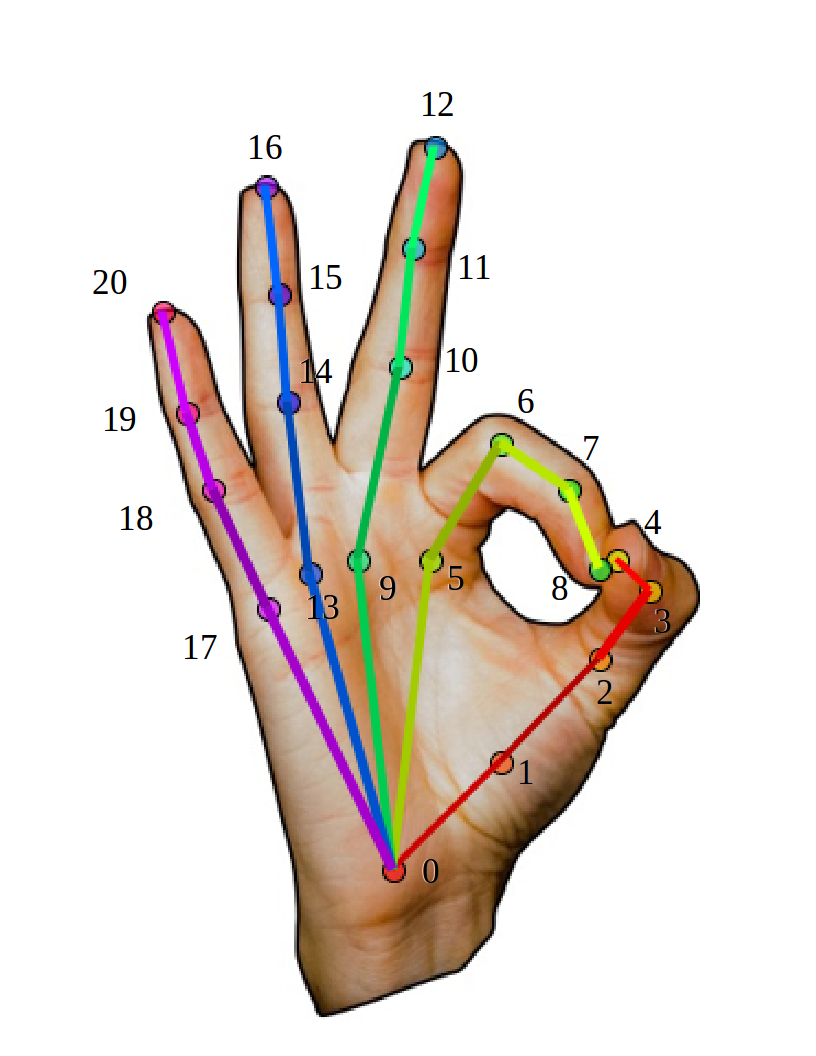
\includegraphics[width=3cm]{images/keypoints_hand}
    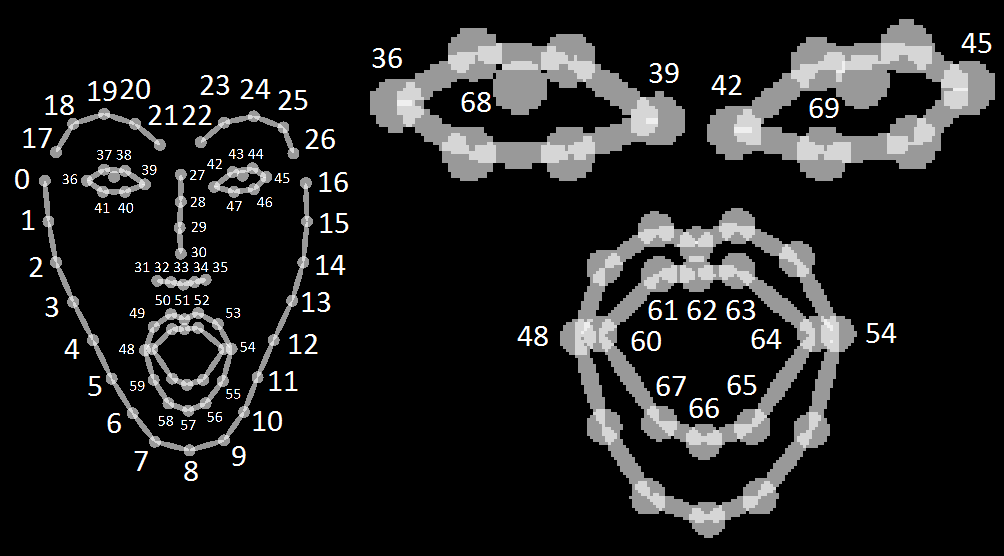
\includegraphics[width=5cm]{images/keypoints_face}
    \caption{Representação dos 21 pontos da mão e 70 pontos da face extraídos pelo OpenPose e que também serão utilizados neste trabalho.}
    \label{fig:keypoints-face-hand}
\end{figure}
Os sinais contidos no \textit{dataset} não possuem sua descrição em CORE-SL e, devido a isso, será necessário produzir suas respectivas \textit{labels} nesse formato. Entretanto, o tempo limitado para execução deste trabalho atua como um dos principais limitadores nessa tarefa e no número de amostras que será possível classificar dessa forma a tempo de aplicar ao modelo e extrair resultados. Algumas estratégias para mitigar esse problemas serão discutidos nas seções seguintes.


\section{Etapas da pesquisa} %%%%%%%%%%%%%%%%%%%%%%%%%%%%%%%%%%%%%%%%%%%
Com o intuito de lidar com os problemas apresentados acima, como a necessidade de criação do  \textit{dataset} em CORE-SL e a demanda por recursos computacionais elevados para execução dos algoritmos de estimação de pose e ST-GCN, esta pesquisa foi segmentada em duas etapas. 

A primeira delas, consiste em atuar na adaptação das camadas de entrada e nas representações internas do modelo ST-GCN para fazê-lo considerar os grafos com os novos pontos do corpo e utilizar a base de dados ASLLVD para seu treinamento. Nesse momento, objetiva-se conhecer o desempenho do modelo frente ao problema da língua de sinais e, dessa forma, os sinais serão classificados segundo seu nome já contido no \textit{dataset} (dispensando a necessidade do \textit{dataset} em CORE-SL). Em termos gerais, essa etapa engloba:
\begin{enumerate}
    \item Localizar \textit{dataset} de língua de sinais (concluído);
    \item Criar pipeline de pré-processamento do \textit{dataset} para o ST-GCN contendo as etapas descritas nas seções anteriores (concluído);
    \item Aumentar o \textit{dataset} para adicionar variações;
    \item Adaptar ST-GCN e suas representações de grafos (em andamento);
    \item Treinar modelo adaptado (em andamento);
    \item Avaliar e melhorar resultados.
\end{enumerate}

Na segunda etapa, as camadas finais do modelo deverão ser adaptadas e a saída do modelo deverá estar no formato das características fonológicas criadas para o novo \textit{dataset} em CORE-SL. Aqui também será necessário definir uma estratégia para representação dessas características pelo classificador. Essa etapa considera os seguintes passos:
\begin{enumerate}
    \item Criar \textit{labels} em CORE-SL para o \textit{dataset}. Para esse passo, considera-se utilizar um subconjunto com cerca de 20 das características mais relevantes do CORE-SL, dado que o conjunto completo contém mais de 100 características;
    \item Definir estratégia para representação das saídas do ST-GCN como CORE-SL;
    \item Adaptar as camadas de saída do ST-GCN para considerar a estratégia acima;
    \item Treinar modelo adaptado;
    \item Avaliar e melhorar resultados.
\end{enumerate}

Atualmente, a pesquisa encontra-se evoluindo em grande parte dos passos estabelecidos para a primeira etapa, sob um ciclo de ajustes, treinamento e otimização.


% Bibliografia
\bibliographystyle{IEEEtran}
\bibliography{IEEEabrv,references.bib}

\end{document}
%%